\section{Présentation Générale}

\subsection{Archétype}

Notre projet sera basé sur le jeu "slay the spire". C'est un jeu de deck building, rogue-like, pour le moment encore en early accesss.



\begin{figure}[h]
\begin{center}
\subfigure{%
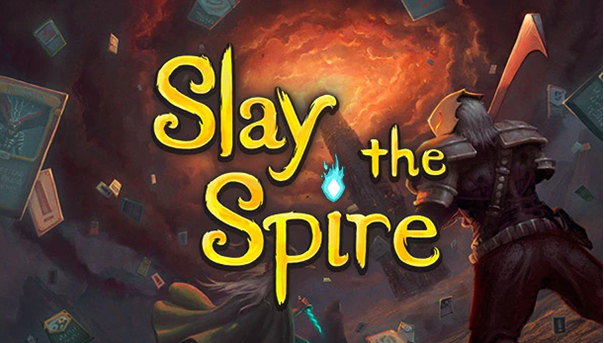
\includegraphics[width=7cm]{images/Welcome_screen.png}}%
\qquad
\subfigure{%
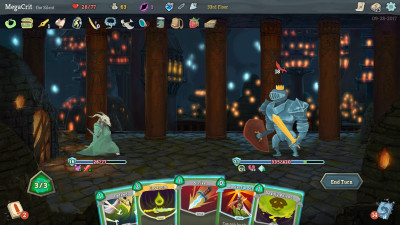
\includegraphics[width=7cm]{images/jeu-ex.jpg}}%
\caption{\label{slaythespiregame}Jeu slay the spire}
\end{center}
\end{figure}

\subsection{Règles du jeu}

Dans ce jeu, le joueur commence avec un deck basique de départ, puis progresse de salle en salle jusqu'à arriver au boss final. Il peut compléter son deck de cartes en fonctions des salles qu'il croise. 

\begin{itemize}
    \item Les salles sont divisées en deux groupes majeurs: les salles d'ennemis, plus fréquentes, et les salles spéciales. Entrer dans une salle d'ennemis déclenche un combat entre le joueur et les ennemis présents dans la salle. Les salles spéciales peuvent avoir des effets positifs ou négatifs sur le joueur. Les effets peuvent être par exemple acquérir une carte puissante, ou obtenir un bonus ou un malus pour le combat suivant.
    \item Le joueur et les ennemis possèdent un nombre de point de vie et une force précise. La puissance des ennemis augmentera avec le nombre de salles parcourues. Vaincre un ennemi consiste à réduire ses points de vie à 0. De même, le joueur perd la partie si sa vie est réduite à 0.
    \item Le deck sera limité à 15 cartes, chaque carte ajoutée doit en remplacer une autre si cette limite est atteinte.
    \item A chaque tour, le joueur possède un taux précis d'énergie et pioche une nouvelle main de 5 cartes. Le joueur peut jouer ses cartes en dépensant de l'énergie, et finir son tour à tout moment. Toutes les cartes non jouées sont défaussées et sont mises dans la pile de défausse. Au tour suivant, toute l'énergie du joueur est regénérée. Il pioche une nouvelle main de 5 cartes issues de sa pioche. Lorsque sa pioche est vide, la défausse du joueur est mélangée et forme la nouvelle pile de pioche. Pendant le tour du joueur, il peut voir les actions qui seront réalisées par les ennemis. Les ennemis jouent toujours leurs actions après le joueur.
    \item Les cartes peuvent être piochées, jouées ou défaussées. Elles dépensent de l'énergie lorsqu'elles sont jouées. Elles peuvent être utilisées pour attaquer l'ennemi, ajouter du block au joueur, ou réaliser d'autres actions plus spécifiques. 
    \item Les cartes et les ennemis possèdent un élément précis (air, eau, terre, feu). Certains éléments seront plus puissants contre d'autres et inversement. Les cartes pourront également apporter des bonus et malus au joueur et aux ennemis.
    \item Les ennemis relachent des cartes après qu'ils soient vaincus, que le joueur peut ajouter à son deck. Ces cartes augmentent en puissance en fonction du nombre de salles parcourues.
    \item Le jeu est découpé en étages et en salles. Chaque étage se termine par un combat de boss, un ennemi plus puissant que les autres, et représentant un élément spécifique. Chaque boss achevé permet la progression du joueur vers l'étage suivant, sauf pour le dernier boss du jeu. Quatres étages, représentant chacun des éléments définis, sont prévus. 
    
\end{itemize}


\subsection{Ressources}

Ressources nécessaires:
\begin{itemize}
    \item Images des joueurs
    
\begin{figure}[H]
\begin{center}
\subfigure{%
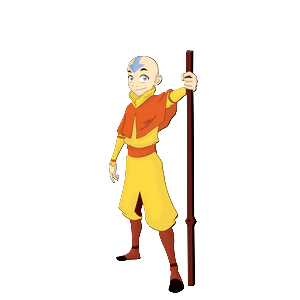
\includegraphics[width=6cm]{images/player/aand.png}}%
\qquad
\subfigure{%
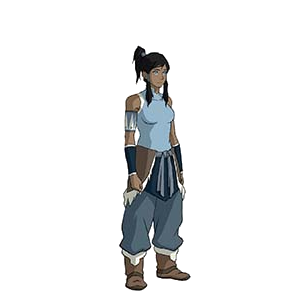
\includegraphics[width=6cm]{images/player/Korra.png}}%
\caption{\label{slaythespiregame}Exemples de deux sprites de joueur}
\end{center}
\end{figure}

\item Image des ennemis

\begin{figure}[H]
\begin{center}
\subfigure{%

\includegraphics[width=3cm]{images/enemy/7.png}}%
\qquad
\subfigure{%

\includegraphics[width=3cm]{images/enemy/bison.png}}%\qquad
\subfigure{%
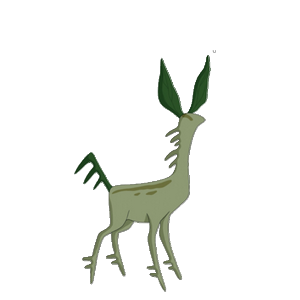
\includegraphics[width=3cm]{images/enemy/19.png}}%
\qquad
\subfigure{%
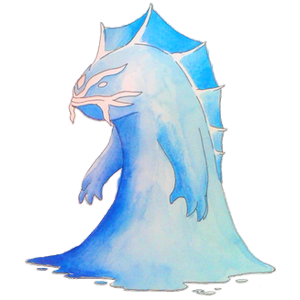
\includegraphics[width=3cm]{images/enemy/La.png}}%
\caption{\label{slaythespiregame}Exemples de sprites d'ennemis}
\end{center}
\end{figure}

\newpage
    \item Fonds pour les salles
    
\begin{figure}[H]
\begin{center}
\subfigure{%
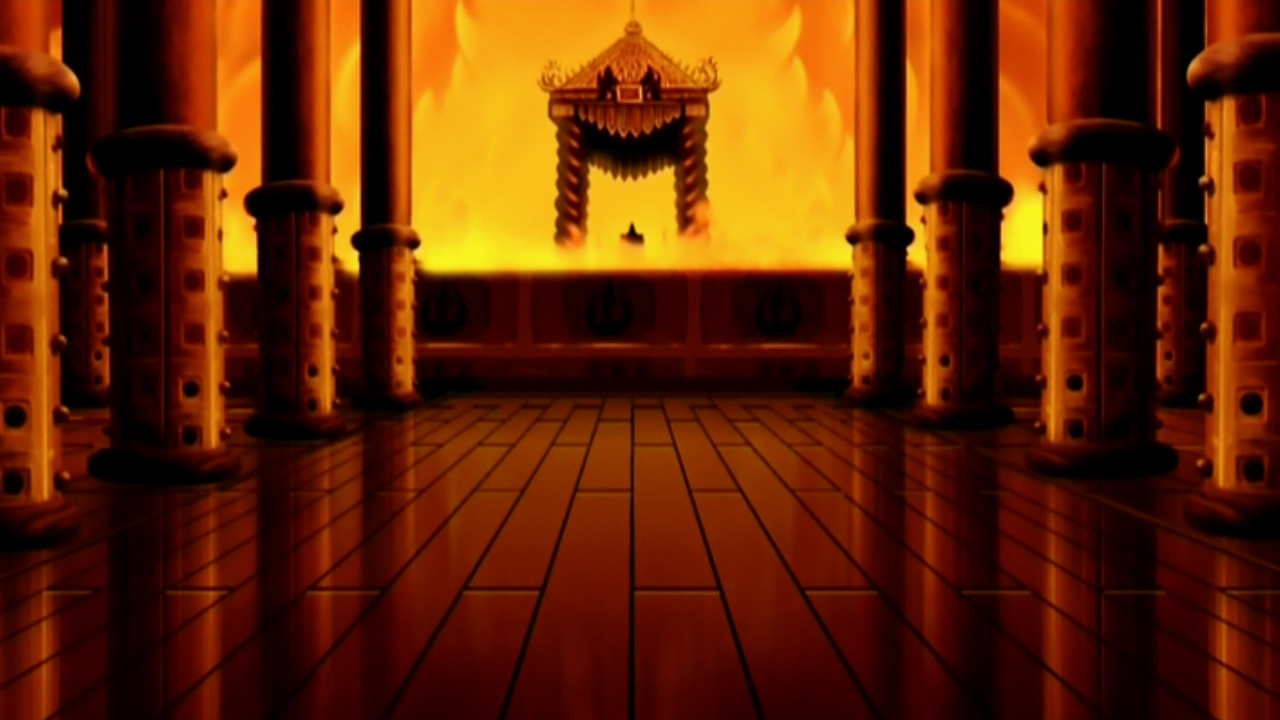
\includegraphics[width=6cm]{images/firenation.jpg}}%
\qquad
\subfigure{%
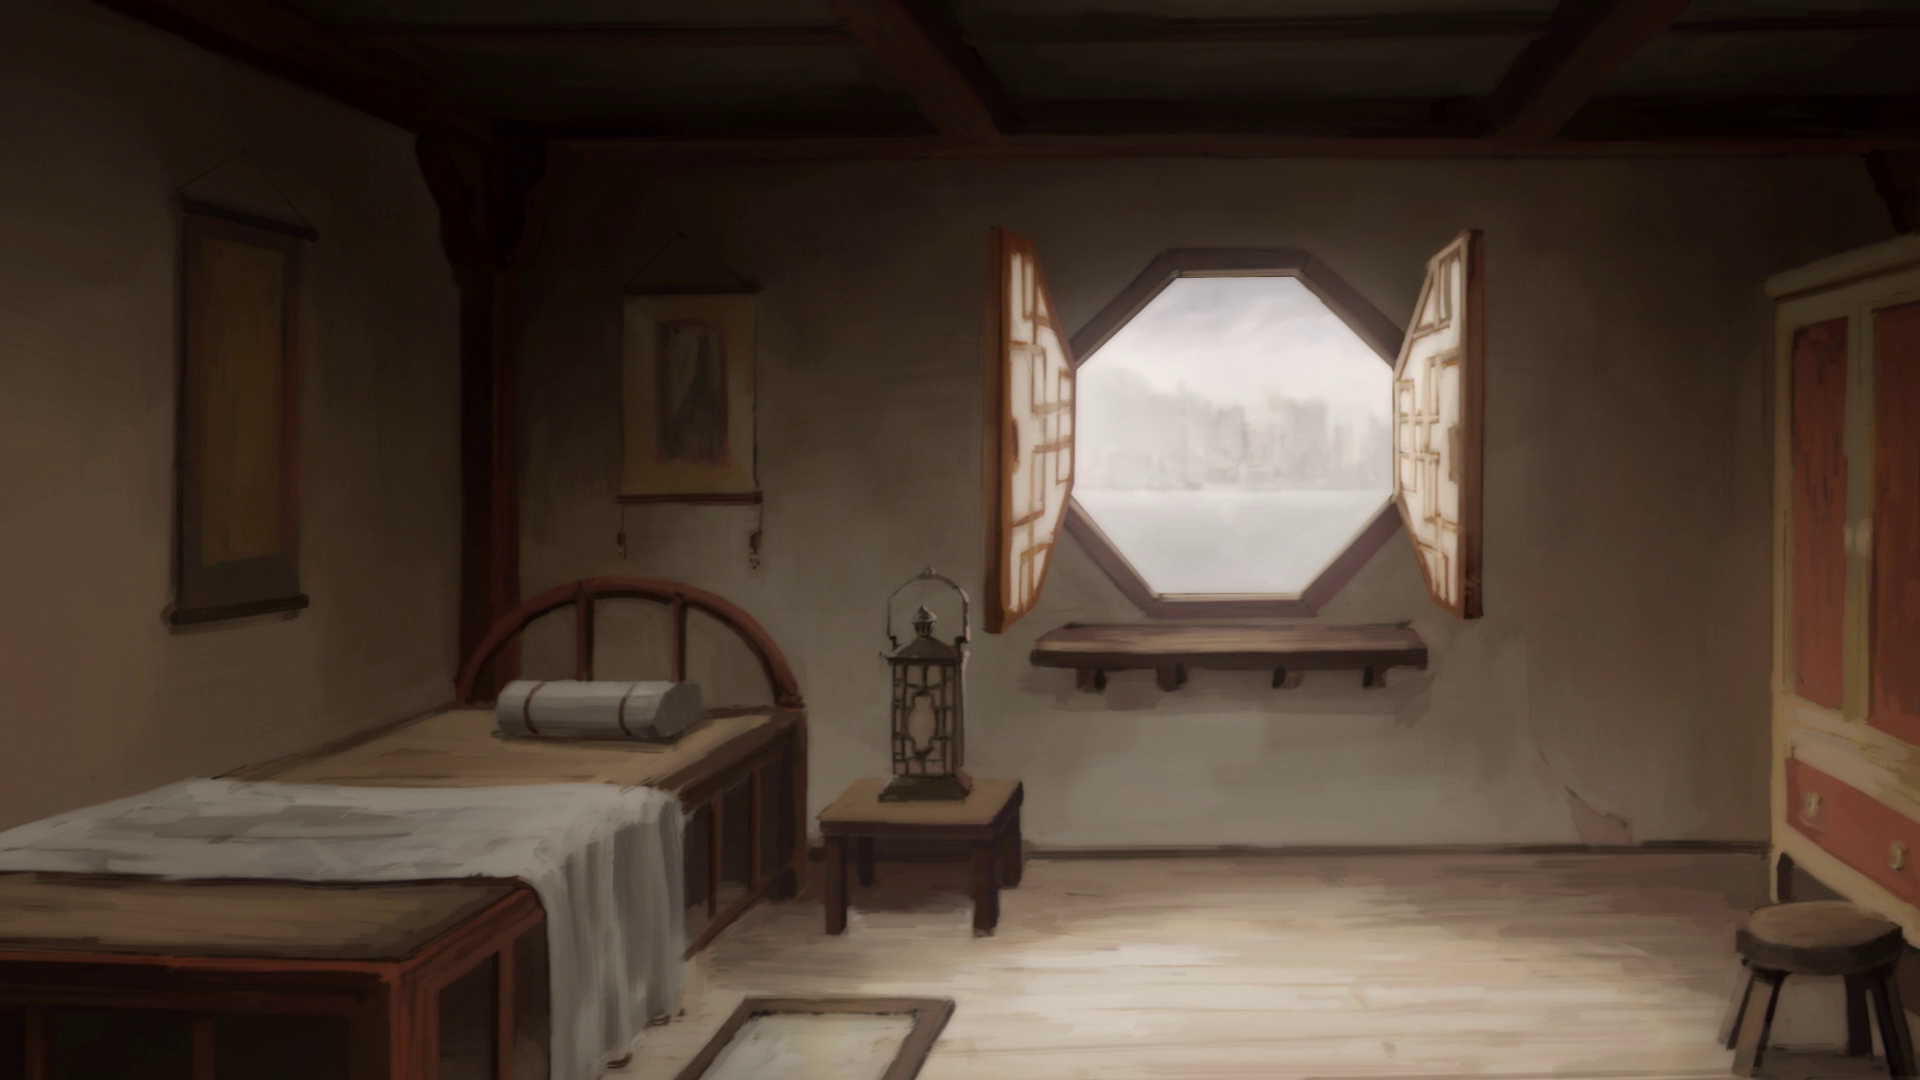
\includegraphics[width=6cm]{images/sleeproom.png}}%
\caption{\label{slaythespiregame}Exemple de deux salles (une salle de combat et une salle de repos}
\end{center}
\end{figure}
    % \newpage
    \item Icones : cartes, bonus/malus, types d'attaque
    
\begin{figure}[H]
\begin{center}
\subfigure{%

\includegraphics[width=1cm]{images/icons/water.png}}%
\qquad
\subfigure{%

\includegraphics[width=1cm]{images/icons/earth.png}}%
\qquad
\subfigure{%

\includegraphics[width=1cm]{images/icons/air.png}}%
\qquad
\subfigure{%

\includegraphics[width=1cm]{images/icons/fire.png}}%
\qquad
\subfigure{%
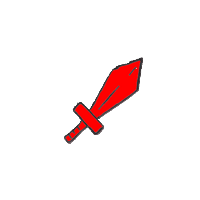
\includegraphics[width=2cm]{images/icons/attack.png}}%
\qquad
\subfigure{%
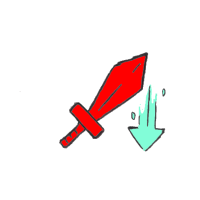
\includegraphics[width=2cm]{images/icons/attack_debuff.png}}%
\qquad
\subfigure{%
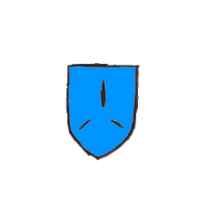
\includegraphics[width=2cm]{images/icons/block.png}}%
\end{center}
\end{figure}

\begin{figure}[H]
\begin{center}
\subfigure{%
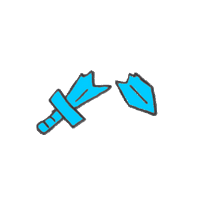
\includegraphics[width=2cm]{images/icons/attack_down.png}}%
\qquad
\subfigure{%

\includegraphics[width=2cm]{images/icons/attack_up.png}}%
\qquad
\subfigure{%
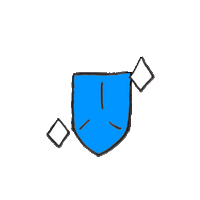
\includegraphics[width=2cm]{images/icons/block_up.png}}%
\qquad
\subfigure{%

\includegraphics[width=2cm]{images/icons/evade.png}}%
\qquad
\subfigure{%

\includegraphics[width=2cm]{images/icons/retaliate.png}}%
\end{center}
\end{figure}

\begin{figure}[H]
\begin{center}
\subfigure{%
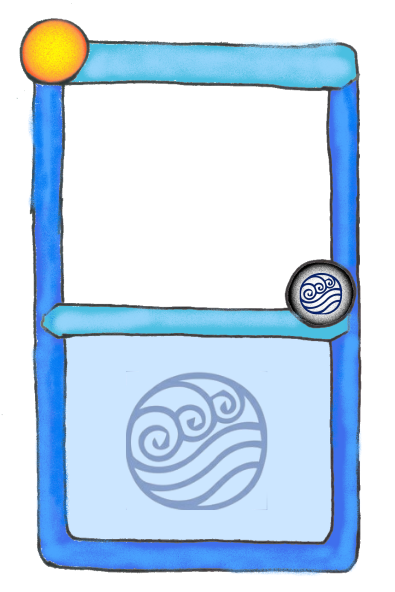
\includegraphics[width=2cm]{images/icons/card_water.png}}%
\qquad
\subfigure{%
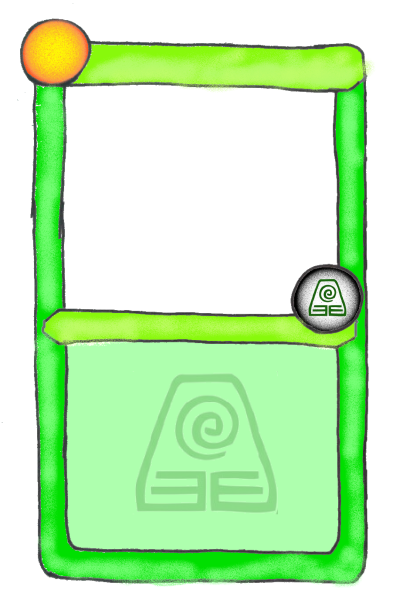
\includegraphics[width=2cm]{images/icons/card_earth.png}}%
\qquad
\subfigure{%
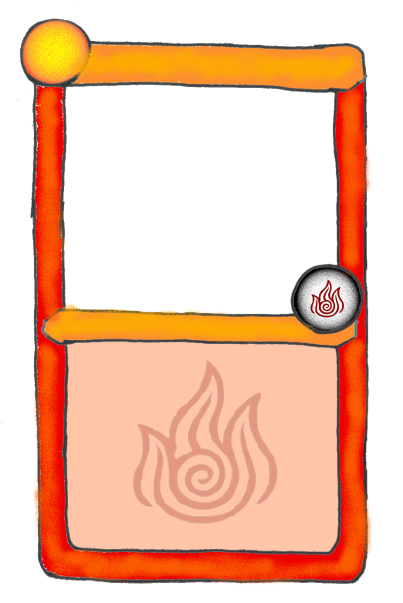
\includegraphics[width=2cm]{images/icons/card_fire.png}}%
\qquad
\subfigure{%
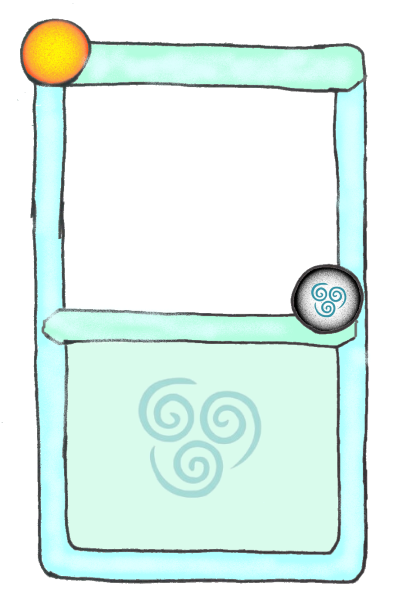
\includegraphics[width=2cm]{images/icons/card_air.png}}%
\qquad
\subfigure{%
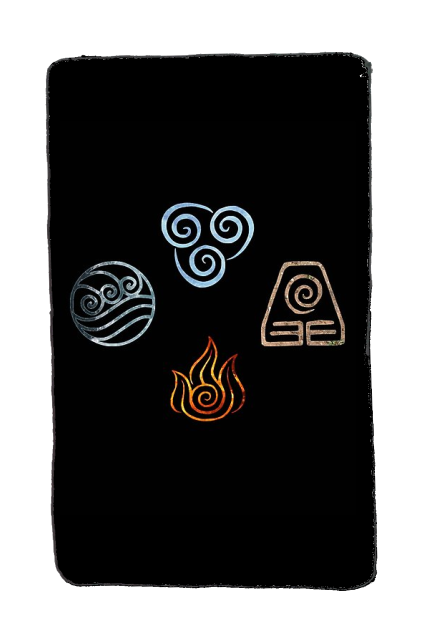
\includegraphics[width=2cm]{images/icons/back_card_fin.png}}%

\caption{\label{slaythespiregame}Exemple de sprites pour les cartes et les différentes icones utilisées}
\end{center}
\end{figure}

% \newpage
    \item Fond de la carte et icones
    
    
\begin{figure}[H]
\begin{center}
\subfigure{%
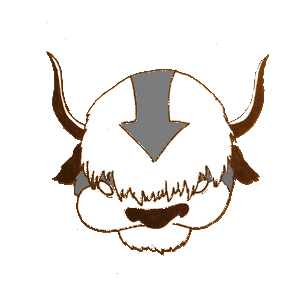
\includegraphics[width=2cm]{images/map/air_bison.png}}%
\qquad
\subfigure{%

\includegraphics[width=2cm]{images/map/air_enemy.png}}%
\qquad
\subfigure{%

\includegraphics[width=2cm]{images/map/fire_enemy.png}}%
\qquad
\subfigure{%
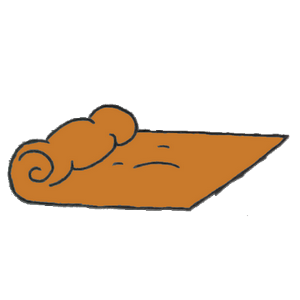
\includegraphics[width=2cm]{images/map/sleep.png}}%
\qquad
\subfigure{%
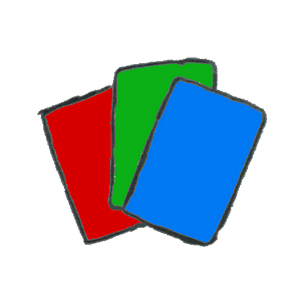
\includegraphics[width=2cm]{images/map/special_training.png}}%
\qquad
\subfigure{%

\includegraphics[width=2cm]{images/map/dragon.png}}%

\caption{\label{slaythespiregame}Exemple d'icones pour la carte}
\end{center}
\end{figure}

\end{itemize}


\clearpage

